% Options for packages loaded elsewhere
\PassOptionsToPackage{unicode}{hyperref}
\PassOptionsToPackage{hyphens}{url}
\PassOptionsToPackage{dvipsnames,svgnames,x11names}{xcolor}
%
\documentclass[
]{krantz}
\title{Graphic Design with ggplot2}
\usepackage{etoolbox}
\makeatletter
\providecommand{\subtitle}[1]{% add subtitle to \maketitle
  \apptocmd{\@title}{\par {\large #1 \par}}{}{}
}
\makeatother
\subtitle{Create Beautiful Data Visualizations in R}
\author{Cédric Scherer}
\date{2022-04-26}

\usepackage{amsmath,amssymb}
\usepackage{lmodern}
\usepackage{iftex}
\ifPDFTeX
  \usepackage[T1]{fontenc}
  \usepackage[utf8]{inputenc}
  \usepackage{textcomp} % provide euro and other symbols
\else % if luatex or xetex
  \usepackage{unicode-math}
  \defaultfontfeatures{Scale=MatchLowercase}
  \defaultfontfeatures[\rmfamily]{Ligatures=TeX,Scale=1}
\fi
% Use upquote if available, for straight quotes in verbatim environments
\IfFileExists{upquote.sty}{\usepackage{upquote}}{}
\IfFileExists{microtype.sty}{% use microtype if available
  \usepackage[]{microtype}
  \UseMicrotypeSet[protrusion]{basicmath} % disable protrusion for tt fonts
}{}
\makeatletter
\@ifundefined{KOMAClassName}{% if non-KOMA class
  \IfFileExists{parskip.sty}{%
    \usepackage{parskip}
  }{% else
    \setlength{\parindent}{0pt}
    \setlength{\parskip}{6pt plus 2pt minus 1pt}}
}{% if KOMA class
  \KOMAoptions{parskip=half}}
\makeatother
\usepackage{xcolor}
\IfFileExists{xurl.sty}{\usepackage{xurl}}{} % add URL line breaks if available
\IfFileExists{bookmark.sty}{\usepackage{bookmark}}{\usepackage{hyperref}}
\hypersetup{
  pdftitle={Graphic Design with ggplot2},
  pdfauthor={Cédric Scherer},
  colorlinks=true,
  linkcolor={Maroon},
  filecolor={Maroon},
  citecolor={Blue},
  urlcolor={Blue},
  pdfcreator={LaTeX via pandoc}}
\urlstyle{same} % disable monospaced font for URLs
\usepackage{color}
\usepackage{fancyvrb}
\newcommand{\VerbBar}{|}
\newcommand{\VERB}{\Verb[commandchars=\\\{\}]}
\DefineVerbatimEnvironment{Highlighting}{Verbatim}{commandchars=\\\{\}}
% Add ',fontsize=\small' for more characters per line
\usepackage{framed}
\definecolor{shadecolor}{RGB}{248,248,248}
\newenvironment{Shaded}{\begin{snugshade}}{\end{snugshade}}
\newcommand{\AlertTok}[1]{\textcolor[rgb]{0.33,0.33,0.33}{#1}}
\newcommand{\AnnotationTok}[1]{\textcolor[rgb]{0.37,0.37,0.37}{\textbf{\textit{#1}}}}
\newcommand{\AttributeTok}[1]{\textcolor[rgb]{0.61,0.61,0.61}{#1}}
\newcommand{\BaseNTok}[1]{\textcolor[rgb]{0.06,0.06,0.06}{#1}}
\newcommand{\BuiltInTok}[1]{#1}
\newcommand{\CharTok}[1]{\textcolor[rgb]{0.5,0.5,0.5}{#1}}
\newcommand{\CommentTok}[1]{\textcolor[rgb]{0.37,0.37,0.37}{\textit{#1}}}
\newcommand{\CommentVarTok}[1]{\textcolor[rgb]{0.37,0.37,0.37}{\textbf{\textit{#1}}}}
\newcommand{\ConstantTok}[1]{\textcolor[rgb]{0,0,0}{#1}}
\newcommand{\ControlFlowTok}[1]{\textcolor[rgb]{0.27,0.27,0.27}{\textbf{#1}}}
\newcommand{\DataTypeTok}[1]{\textcolor[rgb]{0.27,0.27,0.27}{#1}}
\newcommand{\DecValTok}[1]{\textcolor[rgb]{0.06,0.06,0.06}{#1}}
\newcommand{\DocumentationTok}[1]{\textcolor[rgb]{0.37,0.37,0.37}{\textbf{\textit{#1}}}}
\newcommand{\ErrorTok}[1]{\textcolor[rgb]{0.14,0.14,0.14}{\textbf{#1}}}
\newcommand{\ExtensionTok}[1]{#1}
\newcommand{\FloatTok}[1]{\textcolor[rgb]{0.06,0.06,0.06}{#1}}
\newcommand{\FunctionTok}[1]{\textcolor[rgb]{0,0,0}{#1}}
\newcommand{\ImportTok}[1]{#1}
\newcommand{\InformationTok}[1]{\textcolor[rgb]{0.37,0.37,0.37}{\textbf{\textit{#1}}}}
\newcommand{\KeywordTok}[1]{\textcolor[rgb]{0.27,0.27,0.27}{\textbf{#1}}}
\newcommand{\NormalTok}[1]{#1}
\newcommand{\OperatorTok}[1]{\textcolor[rgb]{0.43,0.43,0.43}{\textbf{#1}}}
\newcommand{\OtherTok}[1]{\textcolor[rgb]{0.37,0.37,0.37}{#1}}
\newcommand{\PreprocessorTok}[1]{\textcolor[rgb]{0.37,0.37,0.37}{\textit{#1}}}
\newcommand{\RegionMarkerTok}[1]{#1}
\newcommand{\SpecialCharTok}[1]{\textcolor[rgb]{0,0,0}{#1}}
\newcommand{\SpecialStringTok}[1]{\textcolor[rgb]{0.5,0.5,0.5}{#1}}
\newcommand{\StringTok}[1]{\textcolor[rgb]{0.5,0.5,0.5}{#1}}
\newcommand{\VariableTok}[1]{\textcolor[rgb]{0,0,0}{#1}}
\newcommand{\VerbatimStringTok}[1]{\textcolor[rgb]{0.5,0.5,0.5}{#1}}
\newcommand{\WarningTok}[1]{\textcolor[rgb]{0.37,0.37,0.37}{\textbf{\textit{#1}}}}
\usepackage{longtable,booktabs,array}
\usepackage{calc} % for calculating minipage widths
% Correct order of tables after \paragraph or \subparagraph
\usepackage{etoolbox}
\makeatletter
\patchcmd\longtable{\par}{\if@noskipsec\mbox{}\fi\par}{}{}
\makeatother
% Allow footnotes in longtable head/foot
\IfFileExists{footnotehyper.sty}{\usepackage{footnotehyper}}{\usepackage{footnote}}
\makesavenoteenv{longtable}
\usepackage{graphicx}
\makeatletter
\def\maxwidth{\ifdim\Gin@nat@width>\linewidth\linewidth\else\Gin@nat@width\fi}
\def\maxheight{\ifdim\Gin@nat@height>\textheight\textheight\else\Gin@nat@height\fi}
\makeatother
% Scale images if necessary, so that they will not overflow the page
% margins by default, and it is still possible to overwrite the defaults
% using explicit options in \includegraphics[width, height, ...]{}
\setkeys{Gin}{width=\maxwidth,height=\maxheight,keepaspectratio}
% Set default figure placement to htbp
\makeatletter
\def\fps@figure{htbp}
\makeatother
\setlength{\emergencystretch}{3em} % prevent overfull lines
\providecommand{\tightlist}{%
  \setlength{\itemsep}{0pt}\setlength{\parskip}{0pt}}
\setcounter{secnumdepth}{5}
\usepackage{booktabs}
\usepackage{longtable}
\usepackage[bf,singlelinecheck=off]{caption}
\usepackage[scale=.8]{sourcecodepro}

\usepackage{framed,color}
\definecolor{shadecolor}{RGB}{248,248,248}

\renewcommand{\textfraction}{0.05}
\renewcommand{\topfraction}{0.8}
\renewcommand{\bottomfraction}{0.8}
\renewcommand{\floatpagefraction}{0.75}

\renewenvironment{quote}{\begin{VF}}{\end{VF}}
\let\oldhref\href
\renewcommand{\href}[2]{#2\footnote{\url{#1}}}

\makeatletter
\newenvironment{kframe}{%
\medskip{}
\setlength{\fboxsep}{.8em}
 \def\at@end@of@kframe{}%
 \ifinner\ifhmode%
  \def\at@end@of@kframe{\end{minipage}}%
  \begin{minipage}{\columnwidth}%
 \fi\fi%
 \def\FrameCommand##1{\hskip\@totalleftmargin \hskip-\fboxsep
 \colorbox{shadecolor}{##1}\hskip-\fboxsep
     % There is no \\@totalrightmargin, so:
     \hskip-\linewidth \hskip-\@totalleftmargin \hskip\columnwidth}%
 \MakeFramed {\advance\hsize-\width
   \@totalleftmargin\z@ \linewidth\hsize
   \@setminipage}}%
 {\par\unskip\endMakeFramed%
 \at@end@of@kframe}
\makeatother

\renewenvironment{Shaded}{\begin{kframe}}{\end{kframe}}

\usepackage{makeidx}
\makeindex

\urlstyle{tt}

\usepackage{amsthm}
\makeatletter
\def\thm@space@setup{%
  \thm@preskip=8pt plus 2pt minus 4pt
  \thm@postskip=\thm@preskip
}
\makeatother

\frontmatter
\usepackage{booktabs}
\usepackage{longtable}
\usepackage{array}
\usepackage{multirow}
\usepackage{wrapfig}
\usepackage{float}
\usepackage{colortbl}
\usepackage{pdflscape}
\usepackage{tabu}
\usepackage{threeparttable}
\usepackage{threeparttablex}
\usepackage[normalem]{ulem}
\usepackage{makecell}
\usepackage{xcolor}
\ifLuaTeX
  \usepackage{selnolig}  % disable illegal ligatures
\fi
\usepackage[]{natbib}
\bibliographystyle{apalike}

\begin{document}
\maketitle

% you may need to leave a few empty pages before the dedication page

%\cleardoublepage\newpage\thispagestyle{empty}\null
%\cleardoublepage\newpage\thispagestyle{empty}\null
%\cleardoublepage\newpage
\thispagestyle{empty}

\begin{center}
To my son,

without whom I should have finished this book two years earlier
%\includegraphics{images/dedication.pdf}
\end{center}

\setlength{\abovedisplayskip}{-5pt}
\setlength{\abovedisplayshortskip}{-5pt}

{
\hypersetup{linkcolor=}
\setcounter{tocdepth}{2}
\tableofcontents
}
\listoffigures
\listoftables
\hypertarget{preface}{%
\chapter*{Preface}\label{preface}}


Back in 2016, I had to prepare my PhD introductory talk to inform about my plans for the next three years and to showcase my first preliminary results. I planned to create a visualization using small multiples to show various outcomes of the scenarios I ran with my simulation model. I was already using the R programming language for years and quickly came across the graphics library \textbf{ggplot2} which comes with the functionality to easily create small multiples. I never liked the syntax and style of base plots in R, so I immediately fell in love with the idea and implementation of \textbf{ggplot2}'s \emph{Grammar of Graphics}. But because I was short on time, I plotted these figures by trial and error and with the help of lots of googling. The resource I came always back to was a blog entry called \href{http://zevross.com/blog/2014/08/04/beautiful-plotting-in-r-a-ggplot2-cheatsheet-3/}{``Beautiful plotting in R: A \textbf{ggplot2} cheatsheet'' by Zev Ross}. After giving the talk which contained some decent plots thanks to the blog post, I decided to go through this tutorial step-by-step. I learned so much from it and directly started modifying the codes and adding additional code snippets, chart types, and resources.

Fast forward to 2019. I successfully finished my PhD and started participating in a weekly data visualization challenge called \href{https://github.com/rfordatascience/tidytuesday/blob/master/README.md}{\#TidyTuesday}. Every week, a raw data set is shared with the aim to explore and visualize the data with \textbf{ggplot2}. Thanks to my experience with the \textbf{tidyverse} and especially \textbf{ggplot2} during my PhD and the open-source approach of the challenge that made it possible to learn from other participants, my visualizations quickly became more advanced and complex.

A few months later, I had built a portfolio of various charts and maps and decided to start working as an independent data visualization specialist. I am now using \textbf{ggplot2} every day: for my academic work, design requests, reproducible reports, educational purposes, and personal data visualization projects. What I especially love about my current job specification: It challenges and satisfies my creativity on different levels. Besides the creativity one can express in terms of chart choice and design, there is also creativity needed to come up with solutions and tricks to bring the most venturous ideas to life. At the same time, there is the gratification when your code works and \emph{magically} translates code snippets to visuals.

The blog entry by Zev Ross was not updated since January 2016, so I decided to add more examples and tricks to my version, which was now hosted on my \href{https://www.cedricscherer.com/2019/08/05/a-ggplot2-tutorial-for-beautiful-plotting-in-r/}{personal blog}. Step by step, my version became a unique tutorial that now contains for example also the fantastic \textbf{patchwork}, \textbf{ggtext} and \textbf{ggforce} packages, a section of custom fonts and colors, a collection of R packages tailored to create interactive charts, and several new chart types. The updated version now contains \textasciitilde3.000 lines of code and 188 plots and received a lot of interest from \textbf{ggplot2} users from many different professional fields.

Today, on a sunny day in July 2021, this tutorial serves as the starting point for the book you hold in your hands. I hope you enjoy it as much as I enjoyed learning and sharing \textbf{ggplot2} wizardry!

\hypertarget{why-read-this-book}{%
\section*{Why read this book}\label{why-read-this-book}}


Often, people that use common graphic design and charting tools or have basic experience experience with \textbf{ggplot2} cannot believe what one can achieve with this graphics library---and I want to show you how one can create a publication-ready graphic that goes beyond the traditional scientific scatter or box plot.

\textbf{ggplot2} is already used by a large and diverse group of graduates, researchers, and analysts and the current rise of R and the tidyverse will likely lead to an even increasing interest in this great plotting library. While there are many tutorials on \textbf{ggplot2} tips and tricks provided by the R community, to my knowledge there is no book that specifically addresses the complete design of specific details up to building an ambitious multipanel graphic with \textbf{ggplot2}. As a blend of strong grounding in academic foundations of data visualization and hands-on, practical codes, and implementation material, the book can be used as introductory material as well as a reference for more experienced \textbf{ggplot2} practitioners.

The book is intended for students and professionals that are interested in learning \textbf{ggplot2} and/or taking their default ggplots to the next level. Thus, the book is potentially interesting for \textbf{ggplot2} novices and beginners, but hopefully also helpful and educational for proficient users.

Among other things, the book covers the following:

\begin{itemize}
\tightlist
\item
  Look-up resource for every-day and more specific ggplot adjustments and design options
\item
  Practical hands-on introduction to \textbf{ggplot2} to quickly build appealing visualization
\item
  Discussion of best practices in data visualization (e.g.~color choice, direct labeling, chart type selection) along the way
\item
  Coverage of useful \textbf{ggplot2} extension packages
\item
  Ready-to-start code examples
\item
  Reference implementations illustrating code solutions and design choices
\end{itemize}

\hypertarget{why-r-and-ggplot2}{%
\section*{\texorpdfstring{Why R and \textbf{ggplot2}}{Why R and ggplot2}}\label{why-r-and-ggplot2}}


As a computational ecologist, I've learned and used a range of different tools and programming languages for various purposes such as data wrangling, statistical analyses, and model building. The open-source language R was and is the programming language most widely used by ecologists to handle and analyze ecological data \citep{sciaini2018}. Consequently, I was \emph{of course} using R in my daily life as an scientific researcher.

Nowadays, R plays a crucial part in many data-related workflows, no matter if for scientific, educational, or industrial use cases. Thanks to the ever growing R community and the rich collection of libraries that add additional functionality and simplify workflows, R is an attractive programming language that has outgrown of its original purpose: statistical analyses. Today, R can serve as tool to generate automated reports, develop stand-alone web apps, and draft presentation slides, books, and web pages. And to design high-level, publication--ready visualizations.

Even though R---similar to most programming languages---has a steep learning curve, the level of functionality, flexibility, automation, and reproducibility offered can be a major benefit also in a design context:

\begin{itemize}
\tightlist
\item
  The layered approach of \textbf{ggplot2} opens the possibility to build any type of visualization.
\item
  Various extension packages add missing functionality.
\item
  Script-based workflows instead of \emph{point--and--click} approaches allow for reproducibility---which means you can simply (in theory) run the code again after receiving new data or create thousands of visualizations for various data sets in no time.
\item
  Sharing code is becoming the golden standard in many fields and thus facilitates transparency and credibility as well as modification and creative advancement.
\item
  A helpful community and many free resources simplify learning experiences and the search for solutions.
\item
  The visualizations created in R can be exported as vector files and thus allow for post--processing with graphic design tools.
\end{itemize}

\hypertarget{how-to-read-this-book}{%
\section*{How to read this book}\label{how-to-read-this-book}}


This book can either serve as a textbook or as a reference. Depending on your skill level, some codes and tricks may already be known or not helpful at the moment. In case you want to directly jump to the chapters you find most promising or helpful, here are some suggestions:

\begin{itemize}
\tightlist
\item
  How do I get started with the code? → Chapter \ref{get-started}
\item
  I have no idea how \textbf{ggplot2} actually works and need a quick introduction → Chapter \ref{ggplot}
\end{itemize}

\hypertarget{prerequisites}{%
\section*{Prerequisites}\label{prerequisites}}


To run any of the materials locally on your own machine, you will need the following:

\begin{itemize}
\tightlist
\item
  A recent version of R (download from \href{https://cloud.r-project.org/}{here})
\item
  Preferably an \emph{Integrated Development Environment} (IDE) to store scripts and run code, e.g.~RStudio (download from \href{https://rstudio.com/products/rstudio/download/\#download}{here}) or Visual Studio Code (download from \href{https://code.visualstudio.com/download}{here})
\item
  A set of R packages installed:

  \begin{itemize}
  \tightlist
  \item
    \href{https://www.tidyverse.org/}{\textbf{tidyverse}} that includes \href{https://ggplot2.tidyverse.org/}{\textbf{ggplot2}}
  \item
    \href{https://ggforce.data-imaginist.com/}{\textbf{ggforce}}
  \item
    \href{https://ggrepel.slowkow.com/}{\textbf{ggrepel}}
  \item
    \href{https://wilkelab.org/ggtext/}{\textbf{ggtext}}
  \item
    \href{https://docs.ropensci.org/magick/}{\textbf{magick}}
  \item
    \href{https://patchwork.data-imaginist.com/}{\textbf{patchwork}}
  \item
    \href{https://ragg.r-lib.org/}{\textbf{ragg}}
  \item
    \href{https://docs.ropensci.org/rnaturalearth/}{\textbf{rnaturalearth}}
  \item
    \href{https://github.com/thomasp85/scico}{\textbf{scico}}
  \item
    \href{https://r-spatial.github.io/sf/}{\textbf{sf}}
  \end{itemize}
\end{itemize}

To install all packages in one go, run the following code in the R console:

\begin{Shaded}
\begin{Highlighting}[]
\FunctionTok{install.packages}\NormalTok{(}\FunctionTok{c}\NormalTok{(}
  \StringTok{"tidyverse"}\NormalTok{, }\StringTok{"ggforce"}\NormalTok{, }\StringTok{"ggtext"}\NormalTok{, }\StringTok{"magick"}\NormalTok{, }\StringTok{"patchwork"}\NormalTok{, }
  \StringTok{"ragg"}\NormalTok{, }\StringTok{"rnaturalearth"}\NormalTok{, }\StringTok{"scico"}\NormalTok{, }\StringTok{"sf"}
\NormalTok{))}
\end{Highlighting}
\end{Shaded}

\hypertarget{software-information-and-conventions}{%
\section*{Software information and conventions}\label{software-information-and-conventions}}


The book was written with the \textbf{knitr}\index{knitr} package \citep{xie2015} and the \textbf{bookdown}\index{bookdown} package \citep{R-bookdown} with the following setup:

\begin{verbatim}
## R version 4.1.0 (2021-05-18)
## Platform: x86_64-w64-mingw32/x64 (64-bit)
## Running under: Windows 10 x64 (build 19043)
## 
## Locale:
##   LC_COLLATE=German_Germany.1252 
##   LC_CTYPE=German_Germany.1252   
##   LC_MONETARY=German_Germany.1252
##   LC_NUMERIC=C                   
##   LC_TIME=German_Germany.1252    
## system code page: 65001
## 
## Package version:
##   base64enc_0.1.3   bookdown_0.24    
##   compiler_4.1.0    cpp11_0.4.2      
##   digest_0.6.29     evaluate_0.14    
##   fastmap_1.1.0     glue_1.4.2       
##   graphics_4.1.0    grDevices_4.1.0  
##   highr_0.9         htmltools_0.5.2  
##   jquerylib_0.1.4   jsonlite_1.7.2   
##   knitr_1.36        magrittr_2.0.1   
##   methods_4.1.0     ragg_1.1.3       
##   rlang_0.4.12      rmarkdown_2.11   
##   rstudioapi_0.13   stats_4.1.0      
##   stringi_1.7.5     stringr_1.4.0    
##   systemfonts_1.0.3 textshaping_0.3.6
##   tinytex_0.35      tools_4.1.0      
##   utils_4.1.0       xfun_0.27        
##   yaml_2.2.1
\end{verbatim}

Package names are in bold text (e.g.~\textbf{ggplot2}), and inline code and file names are formatted in a monospaced typewriter font (e.g.~\texttt{read\_csv("data.csv")}). Function names are followed by parentheses (e.g.~\texttt{ggplot2::ggplot()}).

\hypertarget{acknowledgments}{%
\section*{Acknowledgments}\label{acknowledgments}}


Thanks to David Grubbs, Alberto Cairo, Emily Riederer, Oscar Baruffa, and Malcolm Barrett for all your constructive feedback.

\begin{flushright}
Cédric Scherer\\
Berlin, Germany
\end{flushright}

\hypertarget{about-the-author}{%
\chapter*{About the Author}\label{about-the-author}}


Dr Cédric Scherer is a graduated computational ecologist with a passion for good design. In 2020, he combined his expertise in analyzing and visualizing large data sets in R with his interest in design and his perfectionism to become an independent data designer and data visualization consultant.

Cédric has created visualizations across all disciplines, purposes, and styles. Due to regular participation to social data challenges, he is now well known for complex and visually appealing figures, entirely made with ggplot2, that look as they have been created with a vector design tool.

As a data visualization specialist, he does rarely create dashboards but acts as a consultant and designer improving chart and design choices and workshop coach teaching data visualization principles and courses on R and \textbf{ggplot2}. He also uses R and the \textbf{tidyverse} packages to automate data analyses and plot generation, following the philosophy of a reproducible workflow.

\mainmatter

\hypertarget{introduction}{%
\chapter{Introduction}\label{introduction}}

\hypertarget{communicating-data}{%
\section{Communicating Data}\label{communicating-data}}

Communicating data is critical for many of us, no matter if scientists,
journalists, or analysts. How we present data affects the engagement of
and interpretation by the audience. Showing data in an honest,
meaningful---and maybe sometimes even playful or artistic---way is the
art of \textbf{\emph{data visualization}} or \textbf{\emph{information visualization}}. Data
visualization can be described as the transformation of numbers into
visual quantities, encoded by forms, positions, and colors. In the best
case, a well-designed data visualization helps to amplify cognition,
facilitate insights, discover, spark curiosity, explain, and make
decisions.

Data visualizations, or broadly speaking \textbf{\emph{information graphics}}, are
often classified as being either exploratory or explanatory.
\textbf{\emph{Exploratory graphics}} are generated to understand the data and
search for the relevant information. \textbf{\emph{Explanatory graphics}} aim to
communicate the derived information between people
\citep{koponen&hilden2019}. In contrast to exploratory graphics, the creation
of engaging explanatory graphics involves not only the display of data
but also requires many choices with regard to the storytelling and
design.

When designing visualizations myself or looking at the work of others,
the most important question to me is the \textbf{\emph{purpose}} of the graphic.
Without a clear understanding of the purpose, it is impossible to design
an effective and engaging visualization. The same applies when
evaluating a visualization: without the consideration of the
purpose---the audience, the message, the mood---the designer had in mind
when creating the visualization, the critique of design choices often
becomes obsolete. A common assumption is that the single aim of data
visualizations is to guide decisions. This might be true for business or
scientific applications that aim for precision and accuracy by creating
\emph{pragmatic visualizations} \citep{kosara2007}.

At the same time, it is ignorant to assume that efficiency and
functionality are the main purpose of every visualization. Many of the
great visualizations we have seen and that stick to our mind go beyond
the precise, informative display of data\footnote{However, I am not saying that these are the only ones
  that are great---there are definitely several magnificent pragmatic
  visualizations that come to my mind!}. They
experiment with new approaches, use clever, unusual ways to tell stories
or were designed simply to transport joy, curiosity or concern. In some
cases, the design and visual novelty may even be the main focus with the
aim to create a novel, artistic experience for the viewer. Such artworks
are not necessarily created to maximize discovery or communication but
to elicit emotions and can be termed \textbf{\emph{affective
graphics}}\footnote{Credit to the term \textbf{affective graphics} goes to
  Alberto Cairo, thank you for sharing your thoughts with me.}.

As a \emph{creator}, clearly defining the purpose of a visualization helps to
make decisions about the data, the chart type, and the design. As a
\emph{reader}, identifying the purpose helps rating the quality of the
presentation. Some people like to think that there is a single best
approach to visualize data: the one that has survived the test of time
and is the most efficient to quantify information. Some believe that a
chart has to be designed in a *neutral* way. I strongly disagree with
both opinions, for multiple reasons. The most important: Every time we
present the data, we make decisions; and it is not about \emph{if} we make
decisions but \emph{which}. Chart types are not inherently `right' or `wrong'
but might be more or less suitable for the purpose. Colors are
associated with some emotional value---how could we pick one that has a
neutral meaning, association or emotion for every person that might look
at your visualization?

Even if we agree on the `right' decisions---the best chart type and a
neutral color encoding, likely some shades of grey---we still can't
ensure that all people interpret it in the same way. People will always
find their own message in graphs and the interpretation will likely
differ based on individual differences through culture, attitude and
mood.

A quote from Alberto Cairo that is close to my heart sums it up
brilliantly:

\begin{quote}
Visualizations can be designed and experienced in various ways, by
people of various backgrounds, and in various circumstances. That's
why reflecting on the purpose of a visualization is paramount before
we design it---or before we critique it. \citep{cairo2021}
\end{quote}

In the optimal case, the decisions made by the creator are based on some
thoughtful consideration of the following:

\begin{itemize}
\tightlist
\item
  \emph{data} --- which information is meaningful and robust?
\item
  \emph{audience} --- what do readers already know?
\item
  \emph{context} --- how will the reader encounter the visualization?
\item
  \emph{story} --- what is the main message of the visualization?
\item
  \emph{goal} --- which chart type is suitable to transport the story?
\item
  \emph{design} --- how can I facilitate engagement and understanding?
\end{itemize}

While some decisions might (and should) be made before crafting the
visualization, the creation of purposeful, well-designed graphics is an
iterative process. Rarely\footnote{I was very tempted to write ``never'' but I don't have
  data to support this claim\ldots{}} the first draft is what ends
up being printed on physical material or being displayed on your
computer or smartphone screen. Nowadays, computational approaches ease
the cyclic process of prototyping, exploring, testing and designing the
best visual encoding of information for a given purpose.

\hypertarget{coding-visualizations}{%
\section{Coding Visualizations}\label{coding-visualizations}}

As data visualizations involve the quantitative representation of
variables, an environment that allows to handle, wrangle and quantify
data is preferential. Classical design software is great to create
vector-based graphics of all kinds but must often be paired with a
`visualization tool' if the data and/or the chart type becomes more
complex. While there are many tools that allow to quickly create
specific chart types (e.g.~DataWrapper, Flourish, RAWgraphs), often also
with beautiful and very sensible defaults, such chart builder do not
provide full flexibility. Furthermore, the combination of a suite of
tools might be \ldots{}

By using a computational, code-driven approach we can combine all steps
related to data visualization in the same environment: from the data
import and cleaning to the precise and flexible encoding of quantitative
information with custom designs. Programming languages such as
JavaScript, Python, or R have a much steeper learning curve but at the
same time allow users to create almost any visualization one can think
of. Furthermore, they come with several \emph{extension libraries} (e.g.
D3.js, echarts, Vega, Matplotlib, ggplot2) that provide additional
approaches or add more opportunities to existing code.

Data visualizations that are generated with code have several other
benefits. The \emph{reproducibility} of code makes the process more efficient
by being able to update the data or to use the code as a template for
future projects. The \emph{transparency} of coded (and well-documented) data
workflows increases trust. The \emph{scalability} of code allows to produce
the graphics for multiple data sets and use cases.

Of course, the visualization does not need to be created by code alone.
Switching from a code-based approach to a vector-graphics tool makes a
lot of sense in use cases where reproducibility does not matter or
graphics are stand-alone artworks. Honestly, in terms of efficiency and
freedom, a combined approach is likely the best approach in such a case.

With that in mind, knowing how to code visualizations is likely
beneficial in any data-related field.

\hypertarget{get-started}{%
\chapter{Get Started}\label{get-started}}

\hypertarget{data}{%
\section{The Data}\label{data}}

We are using historical data for bike sharing in London in 2015 and 2016, provided by \href{https://tfl.gov.uk/modes/cycling/santander-cycles}{\emph{TfL (Transport for London)}}. The data was collected from the TfL data base and is `Powered by TfL Open Data'. The processed data set contains hourly information on the number of rented bikes and was combined with weather data acquired from freemeteo.com. The data was contributed to the \href{https://www.kaggle.com/hmavrodiev/london-bike-sharing-dataset}{Kaggle online community} by Hristo Mavrodiev.

To make the visualizations manageable and patterns more insightful, we are using a modified data set with all variables aggregated for day (6:00am--5:59pm) and night (6:00pm--5:59am). The bike counts were summarized while all weather-related variables where averaged. Finally, for the weather types, the most common was used and, in case of a tie, one of the most common types was randomly chosen.

\begin{figure}
\centering
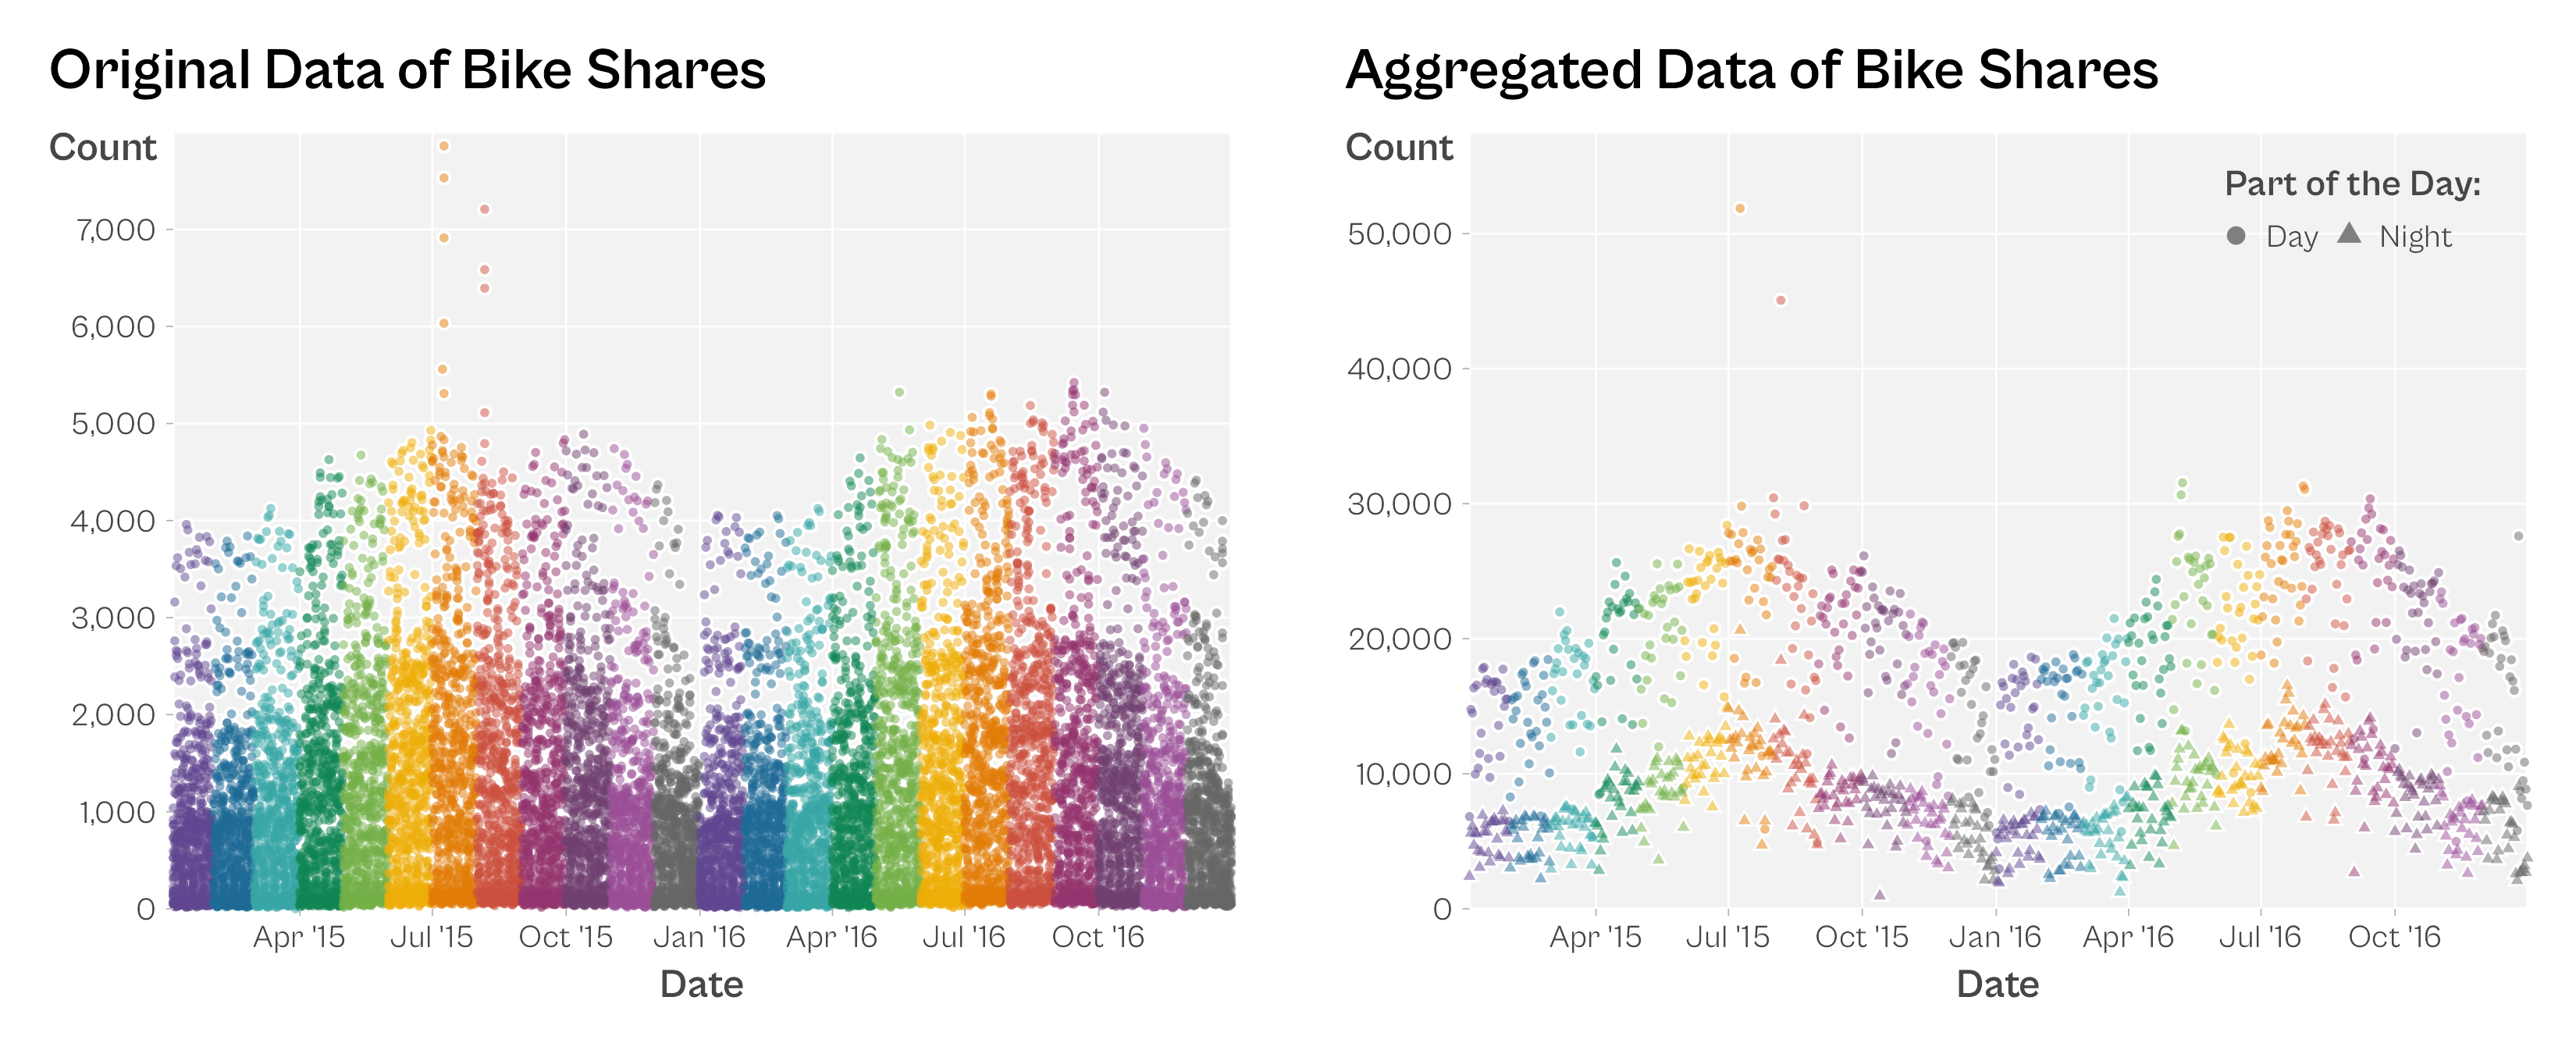
\includegraphics{./img/setup-data-comparison-raw-aggregated.png}
\caption{\label{fig:img-data-comparison}The original and aggregated data sets in direct comparison: counts of bike shares registered by TfL over time with month encoded by colour. The left panel shows counts for every hour of the day, while in the right panel the hourly data was aggregated into two periods of the day (day and night).}
\end{figure}

We can import the data into our R session for example with the \texttt{read\_csv()} function from the \textbf{readr} package. We can import the data set either from a local source or directly from a web URL. To access the data later, we are storing it in a variable called \texttt{bikes} by using the \emph{assignment arrow} \texttt{\textless{}-}. The \texttt{col\_types} argument allows to specify the column types, e.g.~\texttt{i} are integer values, \texttt{f} encodes factors, and \texttt{l} turns a column into logical, boolean variables that are either \texttt{TRUE} or \texttt{FALSE}.

\begin{Shaded}
\begin{Highlighting}[]
\NormalTok{url\_data }\OtherTok{\textless{}{-}} \StringTok{"https://cedricscherer.com/data/london{-}bikes.csv"}
\NormalTok{bikes }\OtherTok{\textless{}{-}}\NormalTok{ readr}\SpecialCharTok{::}\FunctionTok{read\_csv}\NormalTok{(url\_data, }\AttributeTok{col\_types =} \StringTok{"Dcfffilllddddfc"}\NormalTok{)}
\end{Highlighting}
\end{Shaded}

Note: The \texttt{::} is called ``namespace'' and can be used to access a function without loading the package. Here, you could also run \texttt{library(readr)} first and \texttt{bikes\ \textless{}-\ read\_csv(url\_data)} afterwards. Alternatively, you can also use the base R function: \texttt{bikes\ \textless{}-\ read.csv(url\_data)}.

If you inspect the data, e.g.~with the help of \texttt{str()}, \texttt{summary()}, or \texttt{tibble::glimpse()}, you'll see the following 15 variables contained in the data frame with 1454 entries for each:

COMMENT: Decide on a version to provide and overview of the variables as table or list.

\begin{table}

\caption{\label{tab:data-table}Overview of the 15 variables contained in the cleaned and aggregated bike sharing data set.}
\centering
\fontsize{13}{15}\selectfont
\begin{tabular}[t]{llll}
\toprule
Variable & Meaning & Class & Values / Units\\
\midrule
`date` & Date & `date` & `YYYY-MM-DD` format\\
`day\_night` & Period of the day & `character` & day (6:00am–5:59pm) or night (6:00pm–5:59am)\\
`year` & Year & `factor` & `2015` or `2016`\\
`month` & Month as number & `factor` & `1` (January) to `12` (December)\\
`season` & Season as number & `factor` & `0` (spring), `1` (summer), `2` (autumn), or `3` (winter)\\
\addlinespace
`count` & Bike count & `integer` & sum of bikes rented\\
`is\_workday` & Is workday? & `logical` & `TRUE` being Monday to Friday\\
`is\_weekend` & Is weekend? & `logical` & `TRUE` being Saturday or Sunday\\
`is\_holiday` & Is holiday? & `logical` & `TRUE` being an official holiday in the UK\\
`temp` & Air temperature & `double` & average in degree Celsius\\
\addlinespace
`temp\_feel` & Feels like temperature & `double` & average in degree Celsius\\
`humidity` & Humidity & `double` & average in percentage (0-100)\\
`wind\_speed` & Wind speed & `double` & average in kilometres per hour\\
`weather\_code` & Weather type as code & `factor` & most common type\\
`weather\_type` & Weather type as category & `character` & most common type\\
\bottomrule
\end{tabular}
\end{table}

To give you a better idea what the data set contains, here is an graphical overview of the variables contained in the data set and their distributions. Note that I have excluded the variables \texttt{date}, \texttt{year}, \texttt{month}, and \texttt{season} as they are all distributed almost uniform.

\begin{figure}
\centering
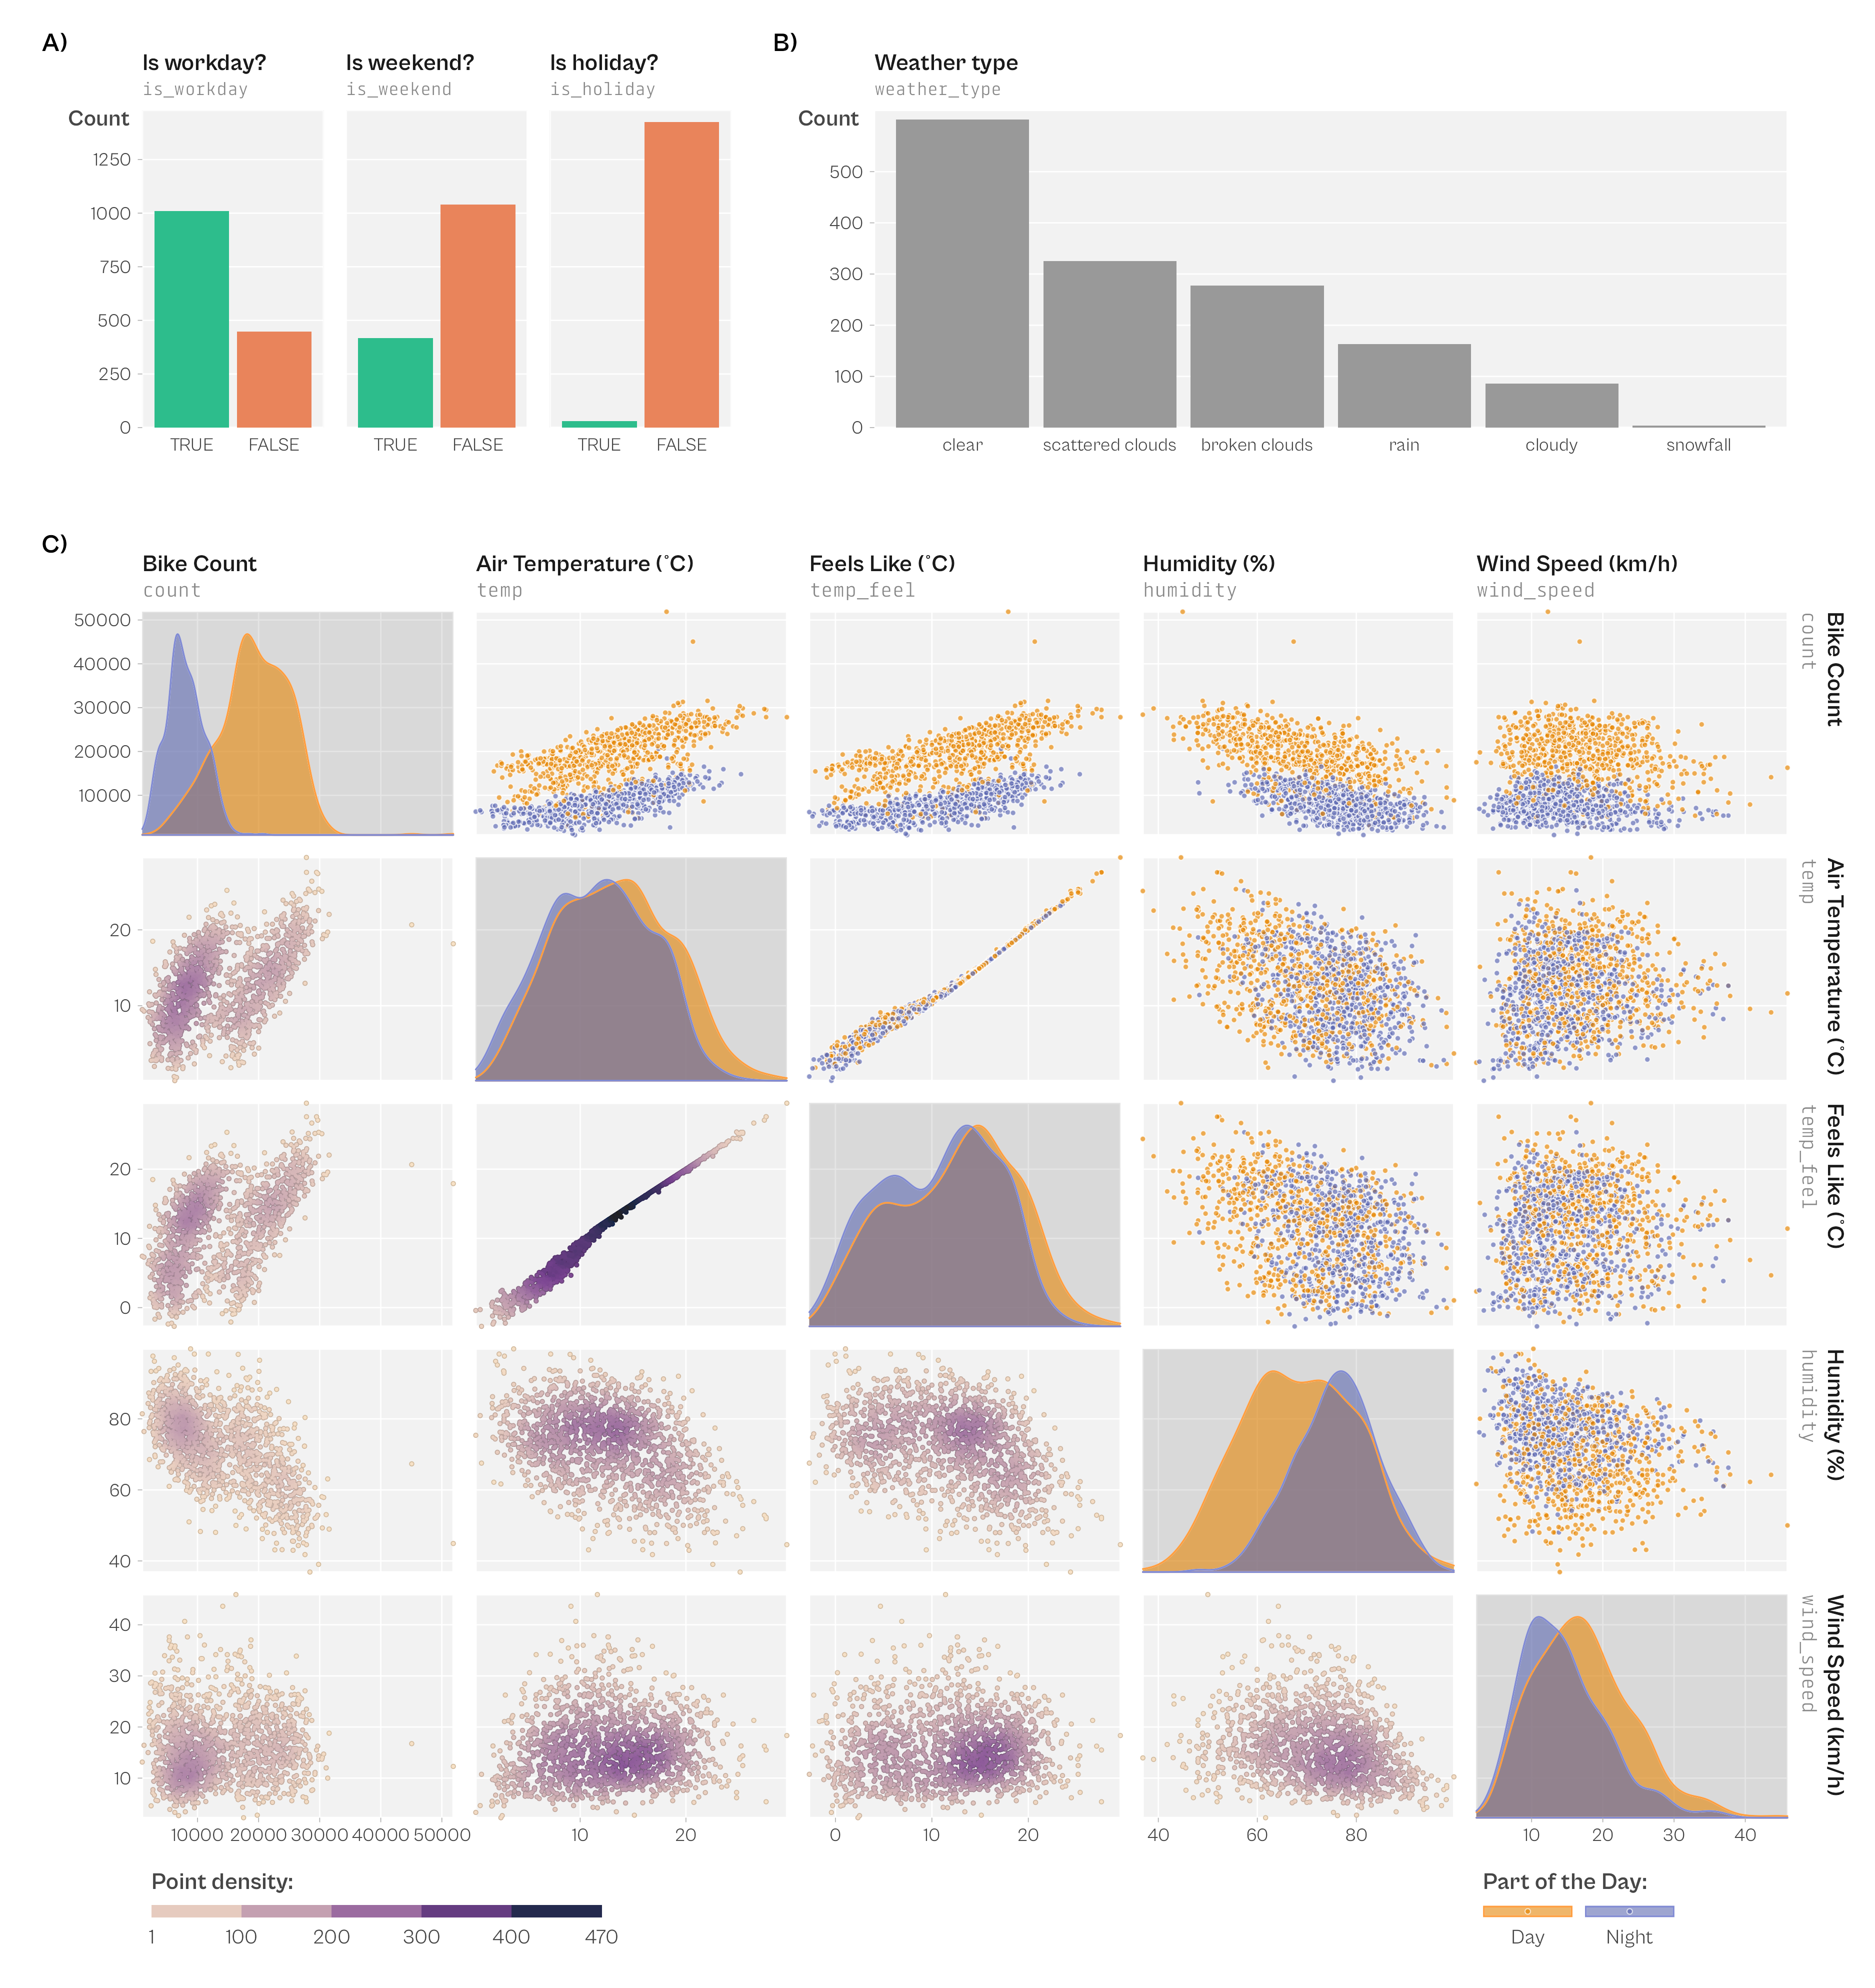
\includegraphics{./img/setup-data-comparison-all-dodge.png}
\caption{\label{fig:img-data-overview-vars}Overview of the distribution of the boolean variables \texttt{is\_workday}, \texttt{is\_weekend}, and \texttt{is\_holiday} (A), the categorical variable \texttt{weather\_type} (B), and the continuous variables \texttt{count}, \texttt{temp}, \texttt{temp\_feel}, \texttt{humidity}, and \texttt{wind\_speed} (C) of the cleaned and aggregated bike sharing data set. In panel C, the correlation between the variables is shown as scatterplot encoded by \texttt{timeperiod} (upper triangle) and encoded by point density (lower triangle), highlighting the level of overlap of data points.}
\end{figure}

COMMENT: A version with overlapping distributions could be used and is available as well.

\hypertarget{rstats}{%
\section{Working in R}\label{rstats}}

\textbf{ggplot2} can be used even if you know little about the R programming language. However, the knowledge of certain basic principles is at least helpful and probably indispensable for advanced plots. This section will give you a short overview of workflows and the

\hypertarget{rmarkdown}{%
\section{Working with Rmarkdown}\label{rmarkdown}}

\hypertarget{ggplot}{%
\chapter{The ggplot2 Package}\label{ggplot}}

ADD SHORT HISTORY OF GGPLOT2

When looking into the package description of the \textbf{ggplot2} package, it states the following:

\begin{quote}
\textbf{ggplot2} is a system for declaratively creating graphics, based on \href{https://link.springer.com/chapter/10.1007/978-3-642-21551-3_13}{The Grammar of Graphics}. You provide the data, tell \textbf{ggplot2} how to map variables to aesthetics, what graphical primitives to use, and it takes care of the details.
\end{quote}

A ggplot is built up from a few components:

\begin{enumerate}
\def\labelenumi{\arabic{enumi}.}
\tightlist
\item
  \textbf{Data}:\\
  The raw data that you want to plot.
\item
  \textbf{Aesthetics} \texttt{aes()}:\\
  Aesthetics that variables are mapped to such as position, color, size, shape, and transparency
\item
  \textbf{Layers:}\\
  The geometric shapes (\texttt{geom\_}) that will represent the data or statistical transformation ( `stat\_`)of the data, such as quantiles, fitted curves, and counts.
\item
  \textbf{Scales} \texttt{scale\_}:\\
  Maps between the data and the aesthetic dimensions, such as data range to positional aesthetics or qualitative or quantitative values to colors.
\item
  \textbf{Coordinate system} \texttt{coord\_}:\\
  The transformation used for mapping data coordinates into the plane of the graphic.
\item
  \textbf{Facets} \texttt{facet\_}:\\
  The arrangement of the data into a grid of plots (also known as \emph{trellis} or \emph{lattice plot}, or simply \emph{small multiples}).
\item
  \textbf{Visual themes} \texttt{theme()}:\\
  The overall visual (non-data) details of a plot, such as background, grid lines, axes, typefaces, sizes, and colors.
\end{enumerate}

Note: The number of elements may vary depending on how you group them and whom you ask. This list is based on the list provided in the \href{https://ggplot2-book.org/introduction.html}{``ggplot2'' book by Hadley Wickham}.

A basic ggplot needs three things that you have to specify: the \emph{data}, \emph{aesthetics}, and a \emph{geometry}. All other components can be added to customize the graphic.

\hypertarget{default}{%
\section{A Basic ggplot}\label{default}}

First, to be able to use the functionality of \textbf{ggplot2} we have to load the package (which we can also load via the \href{https://www.tidyverse.org/}{tidyverse package collection}):

\begin{Shaded}
\begin{Highlighting}[]
\CommentTok{\#library(tidyverse)}
\FunctionTok{library}\NormalTok{(ggplot2)}
\end{Highlighting}
\end{Shaded}

The syntax of \textbf{ggplot2} is very different from plotting functionality of provided by base R. We always start to define a plotting object by calling \texttt{ggplot(data\ =\ df)} which just tells \textbf{ggplot2} that we are going to work with that data. In most cases, you might want to plot two variables---one on the x and one on the y axis. These are \emph{positional aesthetics} and thus we add \texttt{aes(x\ =\ var1,\ y\ =\ var2)} to the \texttt{ggplot()} call (yes, the \texttt{aes()} stands for aesthetics). However, there are also cases where one has to specify only one or even three or more variables.

Note: We specify the data outside \texttt{aes()} and add the variables that ggplot maps the aesthetics to inside \texttt{aes()}.

Here, we map the variable \texttt{date} to the x position and the variable \texttt{temp} to the y position. Later, we will also map variables to all kind of other aesthetics such as color, size, and shape.

\begin{Shaded}
\begin{Highlighting}[]
\FunctionTok{ggplot}\NormalTok{(}\AttributeTok{data =}\NormalTok{ bikes, }\AttributeTok{mapping =} \FunctionTok{aes}\NormalTok{(}\AttributeTok{x =}\NormalTok{ date, }\AttributeTok{y =}\NormalTok{ count))}
\end{Highlighting}
\end{Shaded}

Only a panel is created when running this. Why? This is because \textbf{ggplot2} does not know \emph{how} we want to plot that data---we still need to provide a geometry!

\textbf{ggplot2} allows you to store the current \texttt{ggobject} in a variable of your choice by assigning it to a variable, in our case called \texttt{g}. You can extend this \texttt{ggobject} later by adding other layers, either all at once or by assigning it to the same or another variable.

Note: Thanks to \emph{implicit matching} we can rewrite the code as follows: \texttt{ggplot(bikes,\ aes(date,\ count))}. But be aware that the order matters! I suggest to use a mixture if you feel confident to do so:

\begin{Shaded}
\begin{Highlighting}[]
\FunctionTok{ggplot}\NormalTok{(bikes, }\FunctionTok{aes}\NormalTok{(}\AttributeTok{x =}\NormalTok{ date, }\AttributeTok{y =}\NormalTok{ count))}
\end{Highlighting}
\end{Shaded}

Omitting the arguments \texttt{data} and \texttt{mapping} saves you a ton of typing when creating dozens to hundreds ggplot's per day but being specific about \texttt{x} and \texttt{y} is a good idea. This is the syntax I am using throughout the book.

There are many, many different geometries (called \emph{geoms} because each function usually starts with \texttt{geom\_}) one can add to a ggplot by default (see \href{https://ggplot2.tidyverse.org/reference/}{here} for a full list) and even more provided by extension packages (see \href{https://exts.ggplot2.tidyverse.org/}{here} for a collection of extension packages). Let's tell \textbf{ggplot2} which style we want to use, for example by adding \texttt{geom\_point()} to create a scatter plot:

\begin{Shaded}
\begin{Highlighting}[]
\FunctionTok{ggplot}\NormalTok{(bikes, }\FunctionTok{aes}\NormalTok{(}\AttributeTok{x =}\NormalTok{ date, }\AttributeTok{y =}\NormalTok{ count)) }\SpecialCharTok{+} 
  \FunctionTok{geom\_point}\NormalTok{()}
\end{Highlighting}
\end{Shaded}

\begin{figure}
\centering
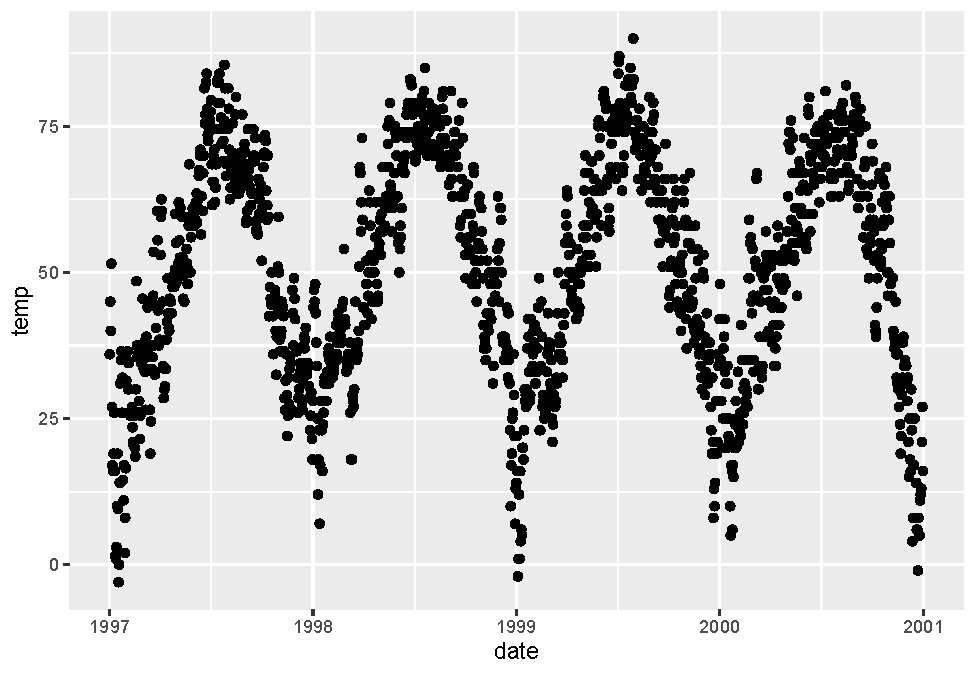
\includegraphics{bookdown_files/figure-latex/ggplot-default-1.png}
\caption{\label{fig:ggplot-default}A default scatter plot of temperature measured in Chicago created with the \textbf{ggplot2} package.}
\end{figure}

One can also combine several geometric layers---and this is where the magic and fun starts!

\begin{Shaded}
\begin{Highlighting}[]
\FunctionTok{ggplot}\NormalTok{(bikes, }\FunctionTok{aes}\NormalTok{(}\AttributeTok{x =}\NormalTok{ date, }\AttributeTok{y =}\NormalTok{ count)) }\SpecialCharTok{+} 
  \FunctionTok{geom\_point}\NormalTok{() }\SpecialCharTok{+} 
  \FunctionTok{geom\_smooth}\NormalTok{()}
\end{Highlighting}
\end{Shaded}

\begin{figure}
\centering
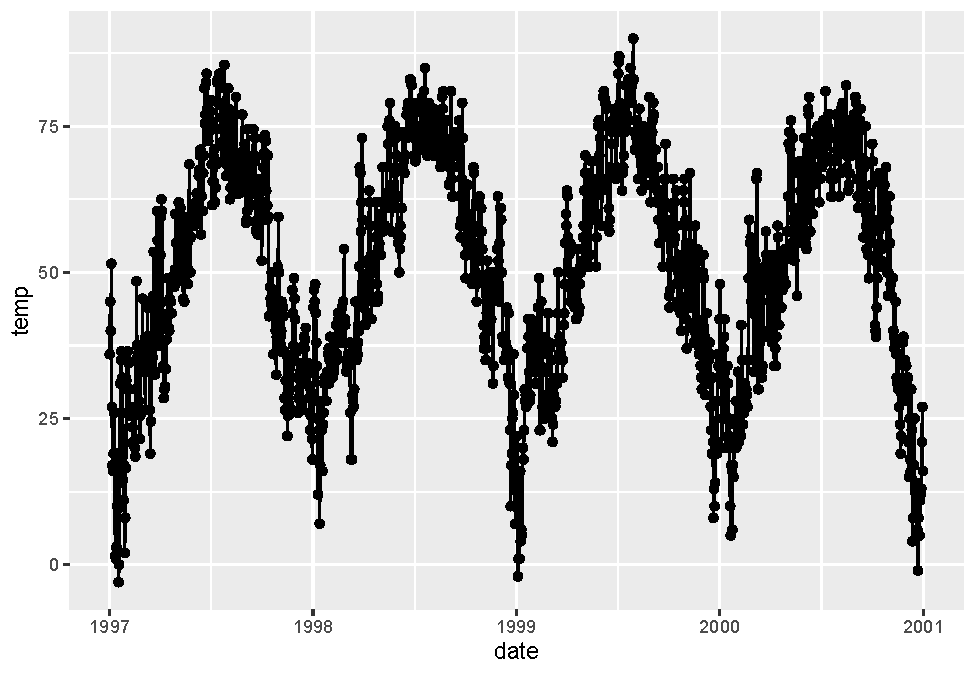
\includegraphics{bookdown_files/figure-latex/ggplot-default-line-point-1.png}
\caption{\label{fig:ggplot-default-line-point}Again, the same data, now shown as a connected scatterplot as a combination of points and lines.}
\end{figure}

That's it for now about geometries. No worries, we are going to learn several plot types in Chapter \texttt{charts}.

\hypertarget{prop}{%
\section{Change Properties of Geometries}\label{prop}}

Within the \texttt{geom\_*} command, you already can manipulate visual aesthetics such as the color, shape, and size of your points. Let's turn all points to large fire-red diamonds!

\begin{Shaded}
\begin{Highlighting}[]
\FunctionTok{ggplot}\NormalTok{(bikes, }\FunctionTok{aes}\NormalTok{(}\AttributeTok{x =}\NormalTok{ date, }\AttributeTok{y =}\NormalTok{ count)) }\SpecialCharTok{+} 
  \FunctionTok{geom\_point}\NormalTok{(}\AttributeTok{color =} \StringTok{"firebrick"}\NormalTok{, }\AttributeTok{shape =} \StringTok{"diamond"}\NormalTok{, }\AttributeTok{size =} \DecValTok{2}\NormalTok{)}
\end{Highlighting}
\end{Shaded}

\begin{figure}
\centering
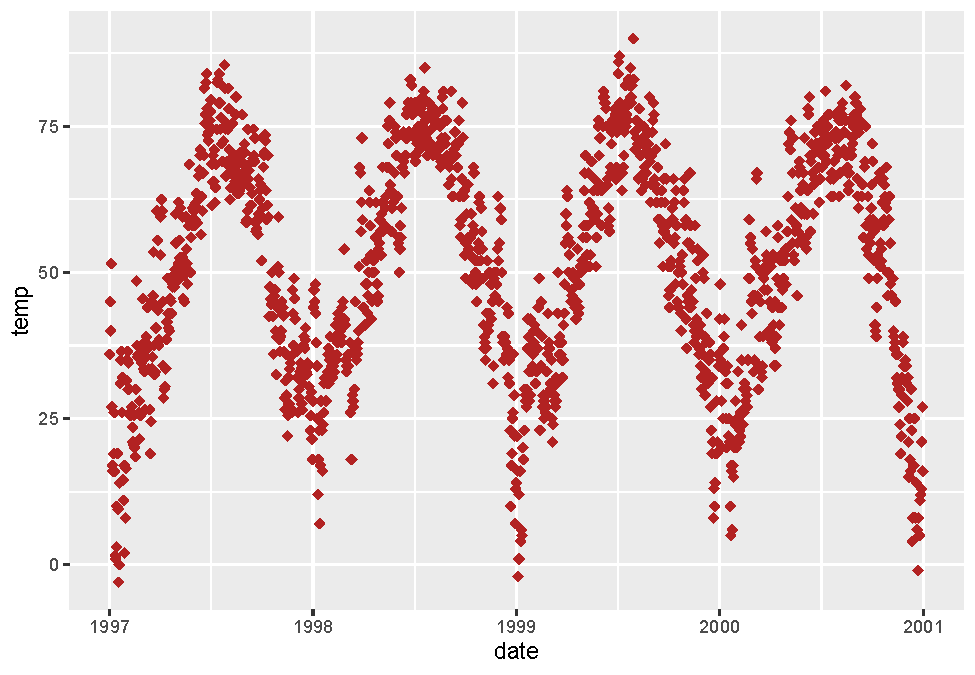
\includegraphics{bookdown_files/figure-latex/ggplot-default-col-size-shape-1.png}
\caption{\label{fig:ggplot-default-col-size-shape}We can change the appearance of the geometry, here illustrated by turning the black dots in larger, red diamonds.}
\end{figure}

\emph{Note: \textbf{ggplot2} understands both \texttt{color} and \texttt{colour} as well as the short version \texttt{col}.}

You can use preset colors (here is a \href{http://www.stat.columbia.edu/~tzheng/files/Rcolor.pdf}{full list}) or \href{https://www.techopedia.com/definition/29788/color-hex-code}{hex color codes}, both in quotes, and even RGB/RGBA colors by using the \texttt{rgb()} function.

\begin{Shaded}
\begin{Highlighting}[]
\FunctionTok{ggplot}\NormalTok{(bikes, }\FunctionTok{aes}\NormalTok{(}\AttributeTok{x =}\NormalTok{ date, }\AttributeTok{y =}\NormalTok{ count)) }\SpecialCharTok{+} 
  \FunctionTok{geom\_point}\NormalTok{(}\AttributeTok{color =} \StringTok{"\#b22222"}\NormalTok{, }\AttributeTok{shape =} \StringTok{"diamond"}\NormalTok{, }\AttributeTok{size =} \DecValTok{2}\NormalTok{)}

\FunctionTok{ggplot}\NormalTok{(bikes, }\FunctionTok{aes}\NormalTok{(}\AttributeTok{x =}\NormalTok{ date, }\AttributeTok{y =}\NormalTok{ count)) }\SpecialCharTok{+} 
  \FunctionTok{geom\_point}\NormalTok{(}\AttributeTok{color =} \FunctionTok{rgb}\NormalTok{(}\DecValTok{178}\NormalTok{, }\DecValTok{34}\NormalTok{, }\DecValTok{34}\NormalTok{, }\AttributeTok{maxColorValue =} \DecValTok{255}\NormalTok{), }\AttributeTok{shape =} \StringTok{"diamond"}\NormalTok{, }\AttributeTok{size =} \DecValTok{2}\NormalTok{)}
\end{Highlighting}
\end{Shaded}

Each geom comes with its own properties (called \emph{arguments}) and the same argument may result in a different change depending on the geom you are using.

\begin{Shaded}
\begin{Highlighting}[]
\FunctionTok{ggplot}\NormalTok{(bikes, }\FunctionTok{aes}\NormalTok{(}\AttributeTok{x =}\NormalTok{ date, }\AttributeTok{y =}\NormalTok{ count)) }\SpecialCharTok{+} 
    \FunctionTok{geom\_point}\NormalTok{(}\AttributeTok{color =} \StringTok{"firebrick"}\NormalTok{, }\AttributeTok{shape =} \StringTok{"diamond"}\NormalTok{, }\AttributeTok{size =} \DecValTok{2}\NormalTok{) }\SpecialCharTok{+} 
    \FunctionTok{geom\_smooth}\NormalTok{(}\AttributeTok{formula =}\NormalTok{ y  }\SpecialCharTok{\textasciitilde{}}\FunctionTok{poly}\NormalTok{(x, }\DecValTok{4}\NormalTok{), }\AttributeTok{se =} \ConstantTok{FALSE}\NormalTok{, }
                \AttributeTok{color =} \StringTok{"gray40"}\NormalTok{, }\AttributeTok{size =} \DecValTok{2}\NormalTok{)}
\end{Highlighting}
\end{Shaded}

\begin{figure}
\centering
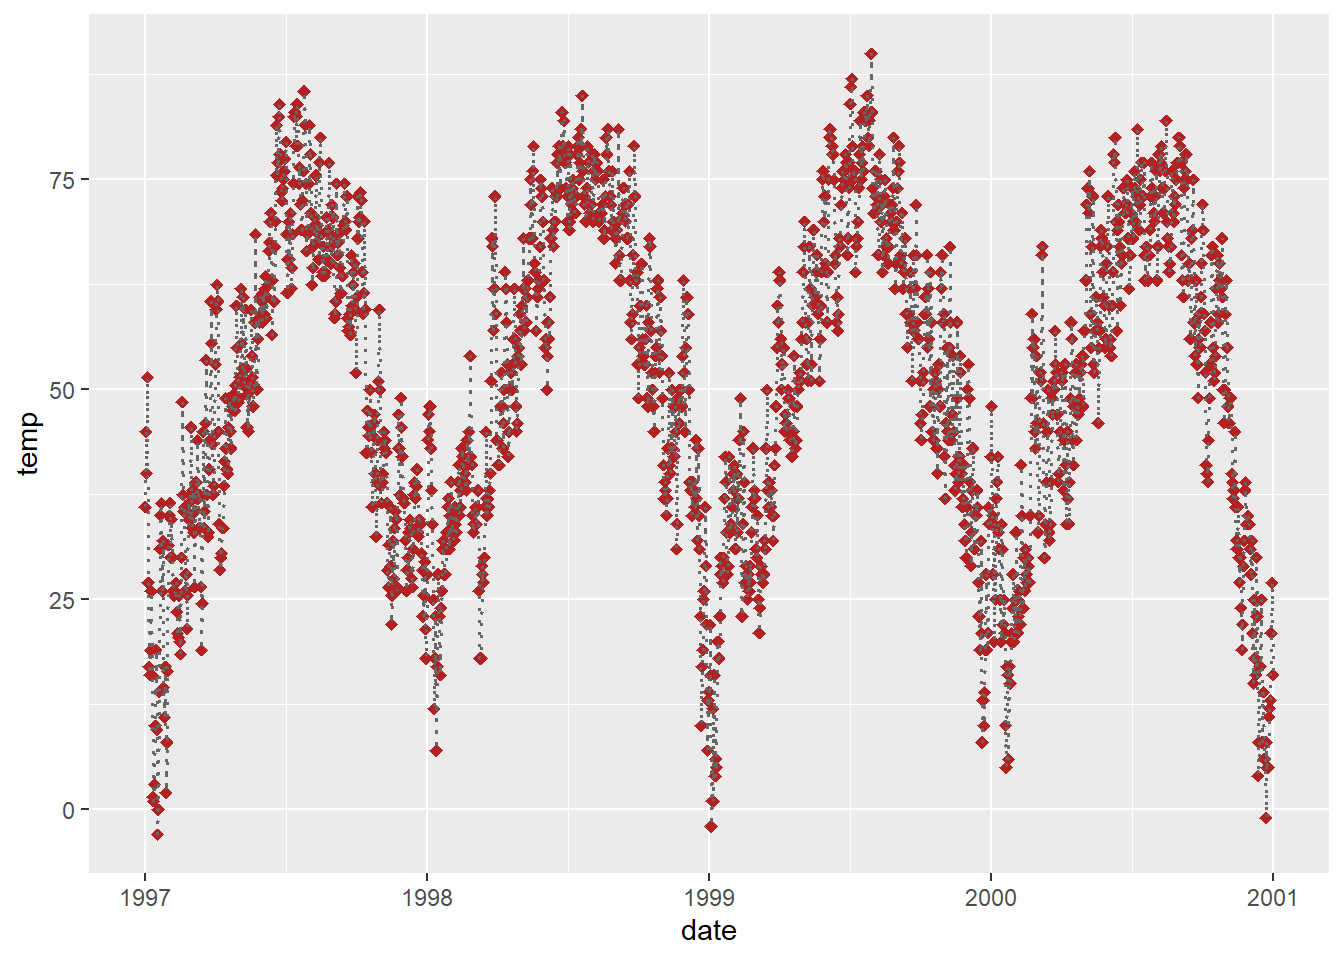
\includegraphics{bookdown_files/figure-latex/ggplot-default-line-col-size-shape-1.png}
\caption{\label{fig:ggplot-default-line-col-size-shape}You can style each geometrical layer on its own. Each geometry also comes with a set of individual properties.}
\end{figure}

\hypertarget{mapping-data-to-aesthetics}{%
\section{Mapping Data to Aesthetics}\label{mapping-data-to-aesthetics}}

You already have seen two \emph{positional aesthetics}, \texttt{x} and \texttt{y} that can be used in combination with the \texttt{aes()} function to map variables to the x- and y-axis, respectively. There are many more aesthetic attributes we are going to use throughout the book. Some are related to positions such as \texttt{ymin} and \texttt{ymax} while others change the appearance of the layer based on the variables they are mapped to such as \texttt{color} and \texttt{shape}.

As with the \texttt{x} and \texttt{y}, the mapping needs to be wrapped into \texttt{aes()} so that ggplot knows that you are referring to columns of your data set. There are two different levels on which you can apply aesthetic mappings: either for all layers or for individual layers only.

In case we want to color our points based on the period of the day to reveal the two patterns, we add \texttt{aes(color\ =\ day\_night)} to our point layer \texttt{geom\_point()}:

\begin{Shaded}
\begin{Highlighting}[]
\FunctionTok{ggplot}\NormalTok{(bikes, }\FunctionTok{aes}\NormalTok{(}\AttributeTok{x =}\NormalTok{ date, }\AttributeTok{y =}\NormalTok{ count)) }\SpecialCharTok{+} 
  \FunctionTok{geom\_point}\NormalTok{(}\FunctionTok{aes}\NormalTok{(}\AttributeTok{color =}\NormalTok{ day\_night)) }\SpecialCharTok{+}
  \FunctionTok{geom\_smooth}\NormalTok{()}
\end{Highlighting}
\end{Shaded}

\begin{figure}
\centering
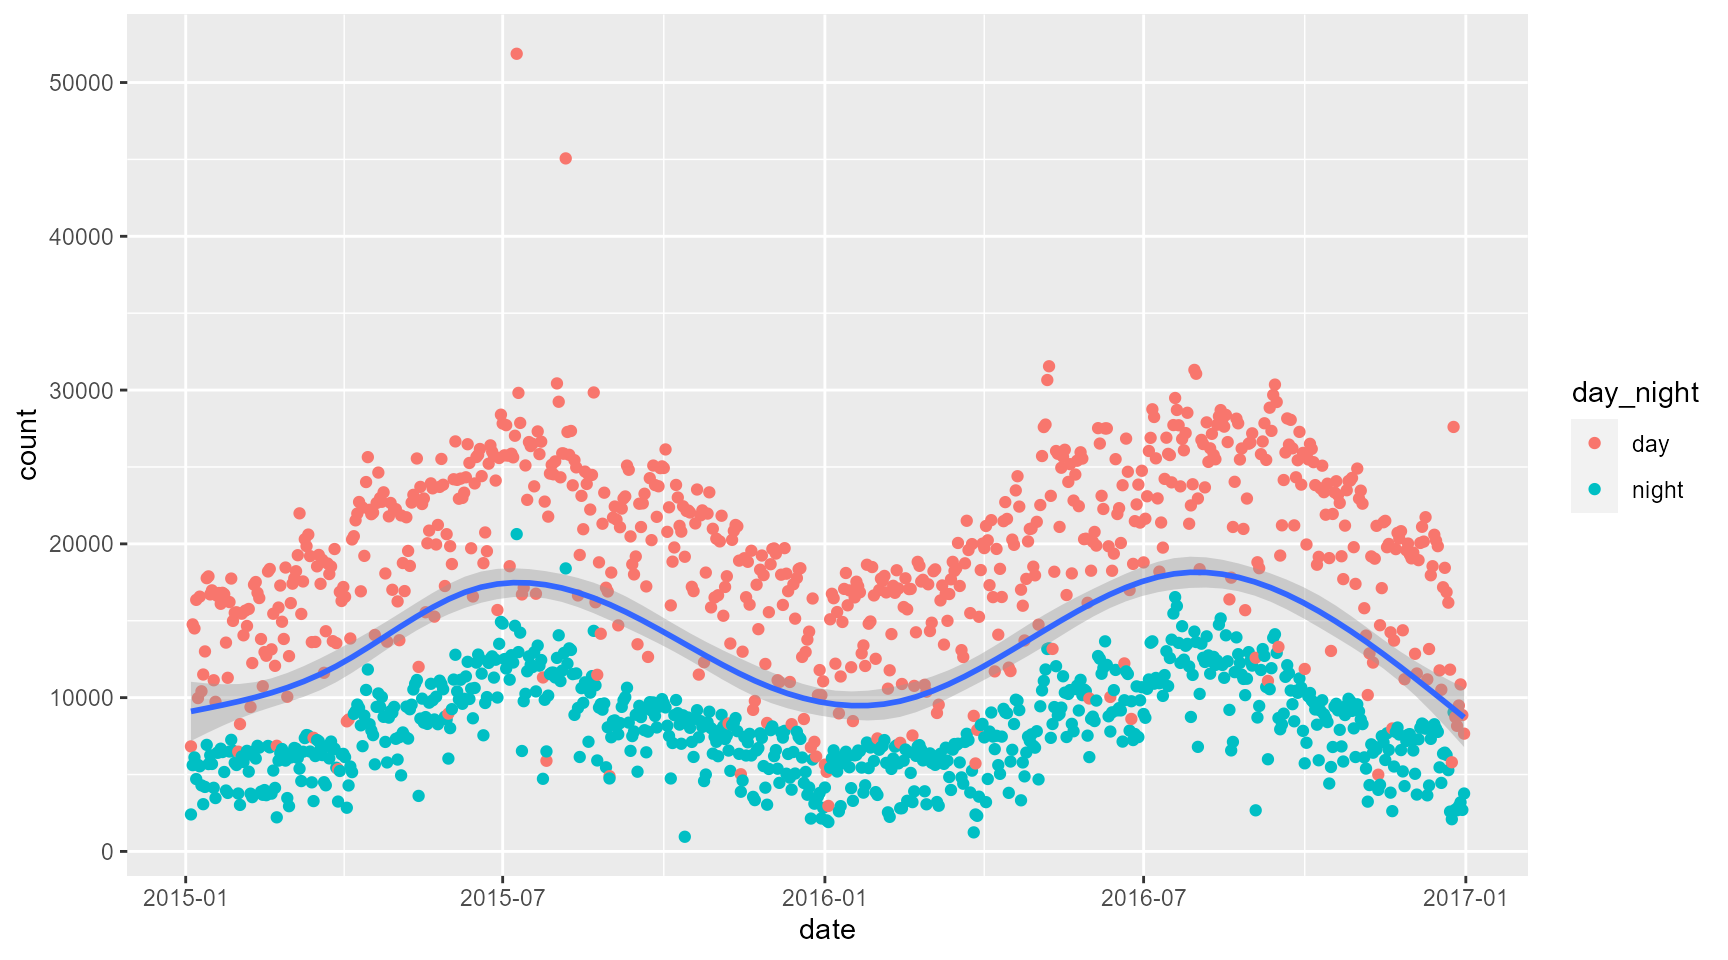
\includegraphics{bookdown_files/figure-latex/ggplot-aes-layer-1.png}
\caption{\label{fig:ggplot-aes-layer}By applying aesthetic mapping to the \texttt{day\_night} variable in the point layers, the two groups can be identified. Note that \textbf{ggplot2} automatically adds a legend to the plot.}
\end{figure}

By supplying the aesthetic mapping inside \texttt{ggplot()} all layers are applying the same mapping. Consequently, the grouping and coloring is also used for the smoothing:

\begin{Shaded}
\begin{Highlighting}[]
\FunctionTok{ggplot}\NormalTok{(bikes, }\FunctionTok{aes}\NormalTok{(}\AttributeTok{x =}\NormalTok{ date, }\AttributeTok{y =}\NormalTok{ count, }\AttributeTok{color =}\NormalTok{ day\_night)) }\SpecialCharTok{+} 
  \FunctionTok{geom\_point}\NormalTok{() }\SpecialCharTok{+}
  \FunctionTok{geom\_smooth}\NormalTok{()}
\end{Highlighting}
\end{Shaded}

\begin{figure}
\centering
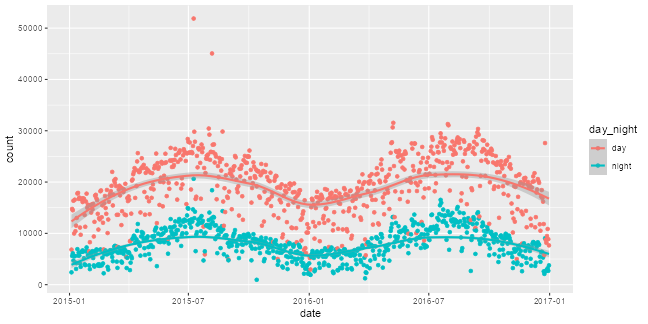
\includegraphics{bookdown_files/figure-latex/ggplot-aes-parent-1.png}
\caption{\label{fig:ggplot-aes-parent}Both, the points and the smoothing lines are encoded by daytime. Because of that, the smoothing is hard to see and best visible in the legend.}
\end{figure}

The aesthetic mapping to both, \texttt{geom\_point()} and \texttt{geom\_smooth()}, is also reflected in the legend which now shows points, lines, and ribbons.

Note that you can overwrite the mapping specified in \texttt{ggplot()} in individual layers by either supplying a fixed value to that property:

\begin{Shaded}
\begin{Highlighting}[]
\FunctionTok{ggplot}\NormalTok{(bikes, }\FunctionTok{aes}\NormalTok{(}\AttributeTok{x =}\NormalTok{ date, }\AttributeTok{y =}\NormalTok{ count, }\AttributeTok{color =}\NormalTok{ day\_night)) }\SpecialCharTok{+} 
  \FunctionTok{geom\_point}\NormalTok{(}\AttributeTok{color =} \StringTok{"black"}\NormalTok{) }\SpecialCharTok{+}
  \FunctionTok{geom\_smooth}\NormalTok{()}

\FunctionTok{ggplot}\NormalTok{(bikes, }\FunctionTok{aes}\NormalTok{(}\AttributeTok{x =}\NormalTok{ date, }\AttributeTok{y =}\NormalTok{ count, }\AttributeTok{color =}\NormalTok{ day\_night)) }\SpecialCharTok{+} 
  \FunctionTok{geom\_point}\NormalTok{() }\SpecialCharTok{+}
  \FunctionTok{geom\_smooth}\NormalTok{(}\AttributeTok{color =} \StringTok{"black"}\NormalTok{)}
\end{Highlighting}
\end{Shaded}

\begin{Shaded}
\begin{Highlighting}[]
\NormalTok{a }\OtherTok{\textless{}{-}} \FunctionTok{ggplot}\NormalTok{(bikes, }\FunctionTok{aes}\NormalTok{(}\AttributeTok{x =}\NormalTok{ date, }\AttributeTok{y =}\NormalTok{ count, }\AttributeTok{color =}\NormalTok{ day\_night)) }\SpecialCharTok{+} 
  \FunctionTok{geom\_point}\NormalTok{(}\AttributeTok{size =}\NormalTok{ .}\DecValTok{5}\NormalTok{, }\AttributeTok{color =} \StringTok{"black"}\NormalTok{) }\SpecialCharTok{+}
  \FunctionTok{geom\_smooth}\NormalTok{()}

\NormalTok{b }\OtherTok{\textless{}{-}} \FunctionTok{ggplot}\NormalTok{(bikes, }\FunctionTok{aes}\NormalTok{(}\AttributeTok{x =}\NormalTok{ date, }\AttributeTok{y =}\NormalTok{ count, }\AttributeTok{color =}\NormalTok{ day\_night)) }\SpecialCharTok{+} 
  \FunctionTok{geom\_point}\NormalTok{(}\AttributeTok{size =}\NormalTok{ .}\DecValTok{5}\NormalTok{) }\SpecialCharTok{+}
  \FunctionTok{geom\_smooth}\NormalTok{(}\AttributeTok{color =} \StringTok{"black"}\NormalTok{)}

\FunctionTok{library}\NormalTok{(patchwork)}
\NormalTok{a }\SpecialCharTok{+} \FunctionTok{plot\_spacer}\NormalTok{() }\SpecialCharTok{+}\NormalTok{ b }\SpecialCharTok{+} \FunctionTok{plot\_layout}\NormalTok{(}\AttributeTok{widths =} \FunctionTok{c}\NormalTok{(}\DecValTok{1}\NormalTok{, .}\DecValTok{02}\NormalTok{, }\DecValTok{1}\NormalTok{))}
\end{Highlighting}
\end{Shaded}

\begin{figure}
\centering
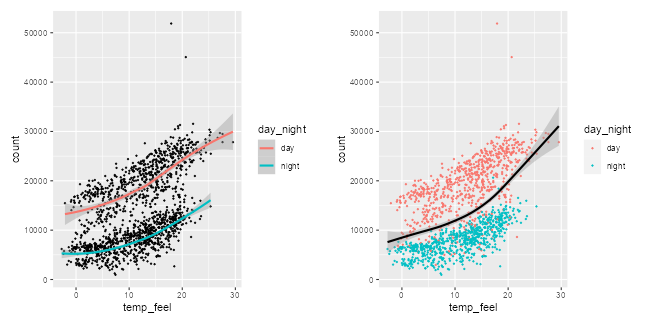
\includegraphics{bookdown_files/figure-latex/ggplot-aes-parent-overwrite-plot-1.png}
\caption{\label{fig:ggplot-aes-parent-overwrite-plot}Overwriting the color encoding in the point (left) or the smoothing (right). Note that the grouping is removed as well which changes the behaviour of the smoothing geom.}
\end{figure}

\hypertarget{theme}{%
\section{\texorpdfstring{Replace the default \textbf{ggplot2} theme}{Replace the default ggplot2 theme}}\label{theme}}

And to illustrate some more of ggplot's versatility, let's get rid of the grayish default \textbf{ggplot2} look by setting a different built-in theme, e.g.~\texttt{theme\_bw()}. One can add a theme directly to a ggplot composition or setting a theme globally---by calling \texttt{theme\_set()} all following plots will have the same black'n'white theme.

\begin{Shaded}
\begin{Highlighting}[]
\FunctionTok{theme\_set}\NormalTok{(}\FunctionTok{theme\_bw}\NormalTok{())}

\FunctionTok{ggplot}\NormalTok{(bikes, }\FunctionTok{aes}\NormalTok{(}\AttributeTok{x =}\NormalTok{ date, }\AttributeTok{y =}\NormalTok{ count, }\AttributeTok{color =}\NormalTok{ day\_night)) }\SpecialCharTok{+} 
  \FunctionTok{geom\_point}\NormalTok{()}
\end{Highlighting}
\end{Shaded}

\begin{figure}
\centering
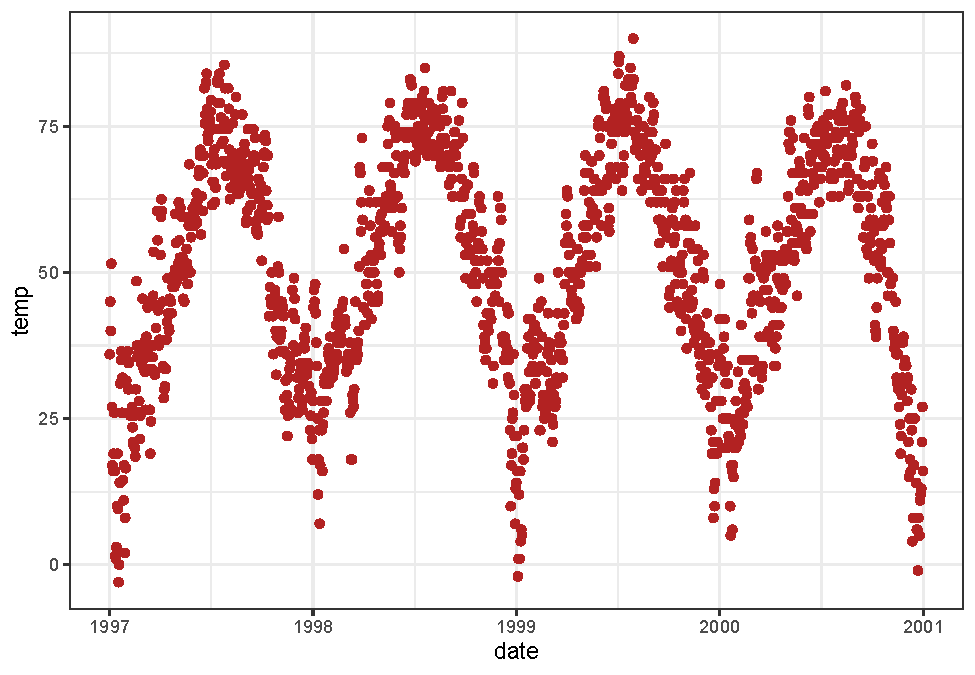
\includegraphics{bookdown_files/figure-latex/remove-gray-background-1.png}
\caption{\label{fig:remove-gray-background}We can change the appearance for all following plots generated with \textbf{ggplot2} by globally setting another theme via \texttt{theme\_set()}.}
\end{figure}

You can find more on how to use built-in themes and how to customize themes in the section \texttt{themes}. From the next chapter on, we will also use the \texttt{theme()} function to customize particular elements of the theme.

\emph{Note: \texttt{theme()} is an essential command to manually modify all kinds of theme elements (texts, rectangles, and lines).}

To see which details of a ggplot theme can be modified have a look \href{https://ggplot2.tidyverse.org/reference/theme.html}{here}---and take some time, this is a looong list.

\cleardoublepage

\hypertarget{appendix-appendix}{%
\appendix \addcontentsline{toc}{chapter}{\appendixname}}


\hypertarget{more-to-say}{%
\chapter{More to Say}\label{more-to-say}}

Yeah! I have finished my book, but I have more to say about some topics. Let me explain them in this appendix.

To know more about \textbf{bookdown}, see \url{https://bookdown.org}.

  \bibliography{book.bib,packages.bib}

\backmatter
\printindex

\end{document}
